\documentclass[journal=jcisd8,manuscript=article]{achemso}

\usepackage{amsmath}
\usepackage{amssymb}
\usepackage{booktabs}
\usepackage{graphicx}
\usepackage{xcolor}
\usepackage{microtype}

\author{Polina Vinogradova}
\affiliation{Independent Researcher}
\altaffiliation{ORCID: 0000-0003-3271-3841}
\email{polina.vino@gmail.com}

\title{Definitional Instability in Kinase Inhibitor Selectivity:
  An Empirical Characterization and Required Properties
  for a Well-Formed Measure}

\abbreviations{S-score, CATDS, pKd, FAERS}
\keywords{binding selectivity, cancer drug discovery,
  cheminformatics, kinase inhibition, research methodology}

\begin{document}

\begin{abstract}
Kinase inhibitor selectivity is quantified using several competing definitions: 
S-score, selectivity entropy, Gini coefficient, and ratio-based measures,
which are applied interchangeably without justification.
Across four profiling datasets spanning three assay technologies (68-704
compounds each), we show these definitions cluster into two families measuring
different properties, and that rank instability is predictable from binding profile shape.
We trace instability to three sources: definitional noise below the detection
threshold, near-tied top targets, and distribution-ratio disagreement for
promiscuous compounds with a dominant target.
We derive four properties that any well-formed selectivity measure should
satisfy, then show that no existing definition satisfies all four. Finally, we propose a
measure that does, recovering its full-panel ranking from about a third of a panel.
\end{abstract}

\noindent\textbf{Keywords:} binding selectivity,
cancer drug discovery, cheminformatics, kinase inhibition, research methodology.

\section{Introduction}
\label{sec:intro}

Kinase inhibitors are among the most intensely investigated compound classes
in drug discovery, with over 80 FDA-approved agents and several hundred in
clinical development.\cite{Roskoski2024}
Because the human kinome is comprised of more than 500 proteins sharing a
highly conserved ATP-binding site,\cite{Manning2002} the design of inhibitors
with controlled target profiles remains a central challenge.
Selectivity is a primary
criterion in lead optimization and a key determinant in the drug approval 
process.\cite{Bhullar2018}

Despite its importance, no single consistent definition of selectivity exists.
The field employs at least four distinct quantitative measures:
the S-score,\cite{Karaman2008} selectivity entropy,\cite{Uitdehaag2011}
Gini coefficient,\cite{Graczyk2010} and ratio-based measures, a family to which
the field assigns the CATDS score.\cite{Klaeger2017}
These definitions are applied interchangeably in the literature without
systematic justification, and their parameter values (the activity threshold
in the S-score, the baseline in the entropy and Gini coefficient, the reference
off-target in ratio-based measures) are chosen by convention rather than
principle.
Standardizing them is a prerequisite for integrating selectivity data across
laboratories and platforms.

Bosc et al.\cite{Bosc2017} showed that these definitions can produce
substantially different compound rankings on the same dataset, and the
KInhibition platform\cite{KInhibition2018} explicitly acknowledged that
conflicting results across metrics are common.
However, the structural sources of this disagreement, such as ``which binding profile
properties determine when definitions agree or conflict, and why?'', have not
been characterized.

The absence of a principled basis for selectivity measurement is not merely
a practical inconvenience. 
Go/no-go decisions in lead optimization are made on the basis of selectivity
assessments whose sensitivity to definitional choice is unknown. The lack of consistency across 
applications of selectivity definitions for different compounds makes 
comparison very challenging. 

Our analyses suggest that existing selectivity definitions are, in some cases,
measuring entirely different qualities of binding profiles, and therefore
cannot be easily converted from one to another. 
In information theory, Shannon\cite{Shannon1948} settled which function should
measure entropy by writing down a few properties a sensible measure must
have (e.g., that it should be maximal when all outcomes are equally
likely) and showing that only one formula satisfies them. In this work, 
we follow this precedent, characterizing how the
competing measures actually behave, stating the properties a good measure
should have, and proposing a satisfactory formula. 

We use four large profiling datasets for kinase inhibitor selectivity
that span three assay technologies in our characterization.
In service of the overarching goal of developing a principled, standardized
formula for defining selectivity, our contributions are as follows:

\begin{itemize}
    \item[(i)] we show that the
S-score, entropy and Gini agree closely with each other on every one of the four
datasets (Spearman $0.72$--$1.00$), while the fold-selectivity ratio $R(k)$
agrees with none of them ($0.14$--$0.62$). We call the first group the
distribution-based family, and $R(k)$ the ratio-based family. The split
follows what each quantifies: how concentrated a compound's activity is across
the whole panel, against how large the gap is to one chosen off-target;

    \item[(ii)] we identify three sources of instability: definitional noise for
compounds with no binding above the activity threshold, ratio-specific instability
driven by near-tied top targets, and distribution-ratio disagreement for
compounds with one dominant target and broad moderate off-target activity;

    \item[(iii)] we propose four motivated properties: (D1) a reliability threshold condition,
(D2) bounded gap sensitivity, (D3) distributional consistency, and (D4) monotonicity under
weak off-target addition. We then find that none of the four definitions
assessed satisfies all four simultaneously;

    \item[(iv)] we propose a candidate measure: a gated, smooth-hinge
effective-target number that satisfies all four properties and recovers its
full-panel ranking from roughly a third of a typical panel.
\end{itemize}

We demonstrate that candidate measure we propose is neither unique as a measure 
satisfying the four properties jointly, nor is it guaranteed to perform better than 
existing measures in all cases. 


\section{Background}
\label{sec:related}

\subsection{Existing Selectivity Metrics and Their Comparison}
\label{sec:related:metrics}

Several metrics have been proposed to quantify kinase inhibitor selectivity
from profiling panel data.
Karaman et al.\cite{Karaman2008} introduced the selectivity score (S-score),
defined as the fraction of panel kinases inhibited above a fixed concentration
threshold.
Uitdehaag and Zaman\cite{Uitdehaag2011} proposed the selectivity entropy,
which treats the normalized binding profile as a probability distribution and
computes its Shannon entropy. Low entropy indicates activity concentrated on
few targets.
Graczyk\cite{Graczyk2010} adapted the Gini coefficient from economics, treating
the distribution of a compound's activity across the panel as an inequality
distribution. A value near 1 indicates activity concentrated on few kinases and
near 0 indicates activity spread evenly.
Klaeger et al.\cite{Klaeger2017} introduced the concentration- and
target-dependent selectivity (CATDS) score, which quantifies the reduction in
binding to a given target relative to the summed reduction across all detected
targets at a specified inhibitor concentration (see Discussion for why we
did not implement it as a fifth measure).
Bosc et al.\cite{Bosc2017} subsequently proposed two further metrics, the
window score and ranking score, and compared them against four previously
published metrics (the S-score, Gini coefficient, selectivity entropy, and a
partition index) on the Davis and Anastassiadis datasets, showing that
compound rankings differ substantially depending on the metric applied and that
certain compounds cannot be scored under some definitions when threshold
conditions are not satisfied. For example, ratio-based scores are undefined
for a compound with no kinase above the activity threshold, since there is then
no primary target or off-target to compare.

Reconciliation attempts have remained limited in scope.
Bajorath et al.\cite{Bajorath2018} compared CATDS-based selectivity
assessments from Klaeger et al.\ with activity data mined from ChEMBL for the
same compounds, finding broad consistency between the two sources.
The KInhibition platform\cite{KInhibition2018} explicitly acknowledged that
multiple existing metrics yield conflicting results for the same compound, but
addressed this by introducing its own composite score (combining on-target
inhibition with an off-target inhibition penalty) rather than reconciling the
disagreement among the existing definitions.
More recently, the same group's built a KIRHub resource\cite{Gujral2026}
on a
new profiling campaign of 86 approved kinase inhibitors against 758 kinases
and disease-associated mutant variants. This resource offers users a choice 
between a further
named metric (the KISS score, an on-target/off-target balance) and a separate
Gini-based score, thus proliferating named, ad hoc definitions.

Two further notable gaps surface in existing work. The first is that
is that each metric is evaluated at fixed
parameter values. Thus, the sensitivity of rankings to parameter choice has not
been systematically characterized. The second i that
the structural properties of binding profiles that determine when definitions
agree or disagree have not been identified.
The present work addresses both gaps.

\subsection{Axiomatic Approaches to Ranking and Measurement}
\label{sec:related:axiomatic}

Precedent for an
axiomatic characterization of measurement functions is established.
Shannon\cite{Shannon1948} demonstrated that the entropy of a probability
distribution is uniquely determined, up to a multiplicative constant, by four
requirements: continuity, maximality on the uniform distribution,
expansibility, and additivity over independent subsystems.
Khinchin\cite{Khinchin1957} subsequently strengthened this uniqueness result.
The selectivity entropy of Uitdehaag and Zaman applies the Shannon formula to
normalized binding profiles but provides no analogous axiomatic justification.
The axioms that single out Shannon entropy, such as maximality on the uniform
distribution and additivity over independent subsystems, characterize a measure
of uncertainty rather than a measure of selectivity.

Arrow\cite{Arrow1951} established that no social welfare function satisfies
simultaneously the requirements of unrestricted domain, Pareto efficiency,
independence of irrelevant alternatives, and non-dictatorship.
The theorem is relevant here in two respects: it demonstrates that axiomatic
analysis of a ranking concept can yield impossibility,
and it shows that competing ranking functions reflect genuine tradeoffs between
properties that cannot all be achieved simultaneously.
Singleton and Booth\cite{Singleton2022} applied this methodology to truth
discovery, i.e. the problem of identifying true facts from conflicting reports of
unknown reliability, posing it as a social choice problem, formulating
candidate axioms, and proving that a subset cannot be jointly satisfied.

To our knowledge, this axiomatic style of analysis has not previously been
applied to any selectivity or promiscuity measure in drug discovery.
The present work proposes empirically motivated properties as a
foundation for such an analysis.

\section{Methods}
\label{sec:methods}

\subsection{Datasets}
\label{sec:methods:data}

Our primary analysis uses two publicly available kinase inhibitor profiling
datasets, described first. Two further datasets are added below to confirm the
findings across additional assay technologies.
The Davis dataset\cite{Davis2011} is comprised of binding affinities ($K_d$) for 68
small-molecule kinase inhibitors measured against 433 human kinase domains.
Affinity values are reported as dissociation constants and were converted to
$\mathrm{p}K_d = -\log_{10}(K_d / 10^9)$ prior to analysis, following the
convention of the DeepDTA benchmark.\cite{DeepDTA}
% Pairs for which no binding was detected at the screening concentration of
% 10~$\mu$M were assigned $\mathrm{p}K_d = 5.0$, corresponding to a $K_d$ of
% 10~$\mu$M, which represents the detection floor of the assay.
The resulting affinity matrix is complete ($68 \times 433$, 29{,}444 entries),
with all non-binding pairs assigned the detection-floor value
$\mathrm{p}K_d = 5.0$ (corresponding to a $K_d$ of 10~$\mu$M).
This is the standard convention for the dataset\cite{DeepDTA,Bosc2017} and
slightly underestimates true non-binding affinity.

Active entries (pKd $> 6$, i.e.\ $K_d < 1~\mu$M) make up 17.9\% of the Davis
matrix. This cutoff answers ``was binding detected above assay noise/floor,''
the conventional boundary used in kinase profiling, rather than ``is this
target plausibly occupied at physiological drug concentrations,'' a question
affinity values alone cannot answer without exposure data (e.g.\ free-drug
concentration) that neither dataset provides. A stricter cutoff
($\mathrm{p}K_d \geq 7$, $K_d < 100$~nM) leaves the agreement between
selectivity definitions unchanged but shrinks per-compound active sets,
pushing more compounds toward the zero/near-zero-active regime that
Section \ref{sec:results:instability} identifies as least rank-stable. 

The Klaeger dataset\cite{Klaeger2017} is comprised of binding affinities for 243
clinical kinase inhibitors profiled against the human kinome using
Kinobeads chemical proteomics.
Apparent dissociation constants ($K_d^\mathrm{app}$) were derived from
dose--response curves across eight inhibitor concentrations in cancer cell
lysates.
Only high-confidence measurements (as annotated by the original authors) were
retained, yielding 5{,}123 drug--target pairs for 222 drugs and 343 kinase
targets.
Affinity values were converted to $\mathrm{p}K_d$ using the same formula as
above.
Missing entries, representing kinase--inhibitor combinations not detected in
the assay, were assigned the background value $\mathrm{p}K_d = 5.0$.
The resulting Klaeger matrix is $222 \times 343$.
Active entries (pKd $> 6$) make up 3.6\% of the Klaeger matrix, versus 17.9\%
for Davis above.
The lower active fraction for Klaeger reflects the more stringent detection
threshold of the chemoproteomic assay.

To test whether our findings depend on the assay technology, we added two
further datasets that measure kinase inhibition by different means.
The Anastassiadis dataset\cite{Anastassiadis2011} profiles 178 inhibitors
against 300 kinases in a single-concentration ($0.5~\mu$M) radiometric activity
assay, reported as percent residual kinase activity relative to a solvent
control.
We converted these to percent inhibition ($100$ minus residual activity,
clipped to $[0,100]$, where higher values denote stronger inhibition), with the
$1.1\%$ missing entries set to zero inhibition.
The Metz dataset\cite{Metz2011} reports $\mathrm{p}K_i$ affinities for a large
medicinal-chemistry
campaign using the same negative-log scale as $\mathrm{p}K_d$. The value
$\mathrm{p}K_i = 4.0$ is the lowest value reported anywhere in the released
data (only $0.17\%$ of measurements), so we assign it to unmeasured
combinations as the assay's own detection floor (the same convention used for
the Davis $\mathrm{p}K_d = 5.0$ floor above). Coverage per compound is highly
skewed (a median compound is measured against only 21 of the 172 kinases), so
we restricted the dataset to the 704 compounds profiled against at least 50 of
the 172 kinases, keeping profiles in which most entries reflect a real
measurement rather than floor imputation while retaining a large enough
compound set for the panel-size and instability analyses.

The four datasets span three assay technologies (competition binding,
chemoproteomics, and functional activity) and two readout types (affinity and
single-concentration inhibition).
Each selectivity definition is computed on the native readout of its
dataset, and our analyses concern rank correlations between definitions and rank
instability. Figure~\ref{fig:fidelity} shows the definitions are not 
invariant to the choice of readout. In fact, two defensible
operationalizations of the entropy rank compounds differently, and on Klaeger in
reverse. Cross-dataset comparison here rests on rank correlations computed within
each dataset, never on absolute scores compared across them.
For the percent-inhibition and $\mathrm{p}K_i$ datasets, the S-score threshold, and
entropy/Gini baseline grids were shifted to span each dataset's active range,
while the ratio off-target index $k \in \{1,\ldots,5\}$ was left unchanged
(it is an index of off-targets and so needs no rescaling).

We excluded two additional candidate datasets.
The Gao screen\cite{Gao2013} is a single-concentration functional inhibition
assay of the same readout type as the Anastassiadis dataset already included,
and its raw data are not openly redistributable. Including it would add a
second instance of an assay type rather than a new assay technology.
The Patricelli study\cite{Patricelli2011} profiles only a small number of
inhibitors against native kinases as a proof of concept for the KiNativ
platform. A ranking-stability analysis requires many compounds to produce a
meaningful ranking, so this dataset is not suited to the present comparison.

\subsection{Selectivity Definitions and Parameterization}
\label{sec:methods:defs}

We implemented four selectivity definitions, each including
parameters whose values are not standardized in the literature.
We discuss each definition below.
Throughout, a compound's binding profile is the vector of its affinities
$\mathrm{p}K_{d,i}$ across the $N$ panel kinases, with higher
$\mathrm{p}K_{d}$ denoting tighter binding.

\paragraph{S-score.}
Karaman et al.\cite{Karaman2008} defined the selectivity score as the fraction
of the panel that a compound inhibits: the number of kinases ``bound'' divided
by the number tested, where a kinase counts as bound when the compound reduces
its activity below a fixed cutoff at a single screening concentration (the
original work reports $S(35)$, $S(10)$ and $S(1)$ for cutoffs of $35\%$, $10\%$
and $1\%$ of control activity).
We implemented the same fraction, expressing the bound criterion as an affinity
threshold $\tau$ on $\mathrm{p}K_d$:
\begin{equation}
  S(\tau) = \frac{1}{N} \sum_{i=1}^{N} \mathbf{1}[\mathrm{p}K_{d,i} > \tau].
\end{equation}
Sweeping $\tau$ reproduces their family of cutoffs. We used
$\tau \in \{5.5, 5.75, \ldots, 8.0\}$ (11 values), spanning $K_d$ cutoffs from
approximately 3~$\mu$M to 10~nM.

\paragraph{Selectivity entropy.}
Uitdehaag and Zaman\cite{Uitdehaag2011} treat the compound's binding across the
panel as a probability distribution and report its Shannon entropy. A profile
concentrated on few kinases has low entropy and is selective.
In the original definition, the weight on each kinase is its association constant
$K_{a,i} = 1/K_{d,i}$ (the share of compound that would be bound to kinase $i$
in an equimolar mixture), so $p_i = K_{a,i}/\sum_j K_{a,j}$.
We implemented the entropy on the same log-affinity scale used by the other
metrics, weighting each kinase by its affinity in excess of a baseline $\beta$:
\begin{equation}
  H(\beta) = -\sum_{i=1}^{N} p_i \log_2 p_i, \quad
  p_i = \frac{\max(\mathrm{p}K_{d,i} - \beta,\, 0)}
             {\sum_j \max(\mathrm{p}K_{d,j} - \beta,\, 0)},
\end{equation}
where $\beta$ is the affinity below which binding is treated as negligible.
This makes $\beta$ an explicit parameter (its under-specification motivates
property D3 below). We swept $\beta \in \{5.0, 5.25, \ldots, 6.5\}$ (7 values),
a narrower range than the S-score's $\tau$ sweep above. Both parameters key off
the same threshold-crossing event, so sweeping either one far enough leaves a
growing share of compounds with no kinase above the cutoff (on Klaeger, 7.2\%
of compounds at $\mathrm{p}K_d = 6.0$ versus 55\% at $\mathrm{p}K_d = 8.0$),
degenerating the S-score toward an uninformative 0 and the entropy and Gini
weights toward an undefined 0/0 alike. The $\tau$ range 
(whose S-score is not necessarily immune to this) is wider because it was 
chosen to reproduce Karaman
et al.'s published cutoffs (approximately 3~$\mu$M to 10~nM). $\beta$ has no
equivalent published reference points and was kept closer to the
$\mathrm{p}K_d = 6$ active threshold used elsewhere in this work.
The association-constant and log-affinity weightings are distinct reasonable
choices that can rank compounds differently, which is itself an instance of the
definitional instability this paper characterizes. We quantify the difference
below. % (``Faithfulness to the original definitions'').

\paragraph{Gini coefficient.}
Graczyk\cite{Graczyk2010} adapted the Gini coefficient from economics: kinases
are sorted by activity and the cumulative fraction of total binding is plotted
against the cumulative fraction of kinases (a Lorenz curve). The Gini
coefficient, which measures how unequally is binding distributed across the kinome,
is twice the area between this curve and the diagonal of equal
distribution.
The original work computes it from percent-inhibition values.
As with the entropy above, implemented the entropy on the same log-affinity scale
for the same reason.
We applied the standard discrete Gini formula to that baseline-subtracted
log-affinity profile:
\begin{equation}
  G(\beta) = \frac{2\sum_{i=1}^{N} i \cdot x_{(i)}}{N \sum_{i=1}^{N} x_{(i)}} - \frac{N+1}{N},
  \qquad x_{(i)} = \max(\mathrm{p}K_{d,i} - \beta,\, 0)\  \text{sorted ascending}.
\end{equation}
We swept $\beta$ over the same range as for the entropy.
A compound whose binding is concentrated on one kinase has a highly unequal
distribution ($G$ is near 1), while a compound that binds many kinases equally has
$G$ near 0. Higher values therefore indicate greater selectivity.

\paragraph{Ratio.}
Classical pharmacological selectivity is pairwise. It quantifies how much more tightly a
compound binds its primary target than an off-target.
We implemented this as the fold-selectivity, in log units, between the primary
target and the $k$-th ranked off-target:
\begin{equation}
  R(k) = \mathrm{p}K_{d,(1)} - \mathrm{p}K_{d,(k+1)}
       = \log_{10}\frac{K_{d,(k+1)}}{K_{d,(1)}},
\end{equation}
where $\mathrm{p}K_{d,(j)}$ is the $j$-th largest affinity in the profile and
$k \in \{1, 2, 3, 4, 5\}$ selects the reference off-target. We capped $k$ at 5
because, on the sparser Klaeger panel, a large share of compounds already have
fewer than five active kinases (median 5.5; $45\%$ have fewer than five). For
those compounds, a larger $k$ would compare the primary target against the
assay floor rather than a genuine off-target.
$R(k)$ takes
the affinity gap to a single chosen competitor, the $k$-th ranked off-target.
The field also assigns the concentration- and target-dependent selectivity
(CATDS) score of Klaeger et al.\cite{Klaeger2017} to this family, though we find
that it does not behave like a member of it. CATDS divides each
target's concentration-dependent binding reduction by the sum of binding
reductions over \emph{every} target in the panel, rather than comparing to a
single chosen competitor, which is a distributional construction. We therefore
represent the ratio family by $R(k)$ alone and treat CATDS separately in the
Discussion.
We use the simpler fold-selectivity because the reference off-target index $k$
is then an explicit parameter whose effect can be studied directly.
A larger affinity gap to the nearest competitor means greater selectivity, so
higher $R(k)$ indicates greater selectivity.
% \emph{In words:} how big is the affinity gap between the primary target and the
% next-best one? A larger gap means greater selectivity.

\paragraph{Faithfulness to the original definitions.}
The S-score and the ratio are computed in the form given by their original
sources (a panel-hit fraction and a primary-to-off-target affinity ratio,
respectively).
For the entropy and the Gini coefficient, we used the baseline-subtracted
log-affinity profile in place of the original association constants (entropy)
and percent-inhibition values (Gini), so that all four metrics operate on one
common scale, and making baseline $\beta$ an explicit calculation parameter.
To confirm that this choice does not implicitly determine our conclusions, we
recomputed the entropy and Gini in forms closer to the originals
(association-constant weighting) and compared the resulting rankings with the
log-affinity forms.
The two operationalizations differ substantially: for entropy, Spearman
$r = 0.42$ (Davis) and $-0.32$ (Klaeger), while for Gini, $r = 0.11$ and $-0.45$
(Figure~\ref{fig:fidelity}). This confirms that the operationalization
of a named metric is a source of the definitional instability.

\begin{figure}[htbp]
  \centering
  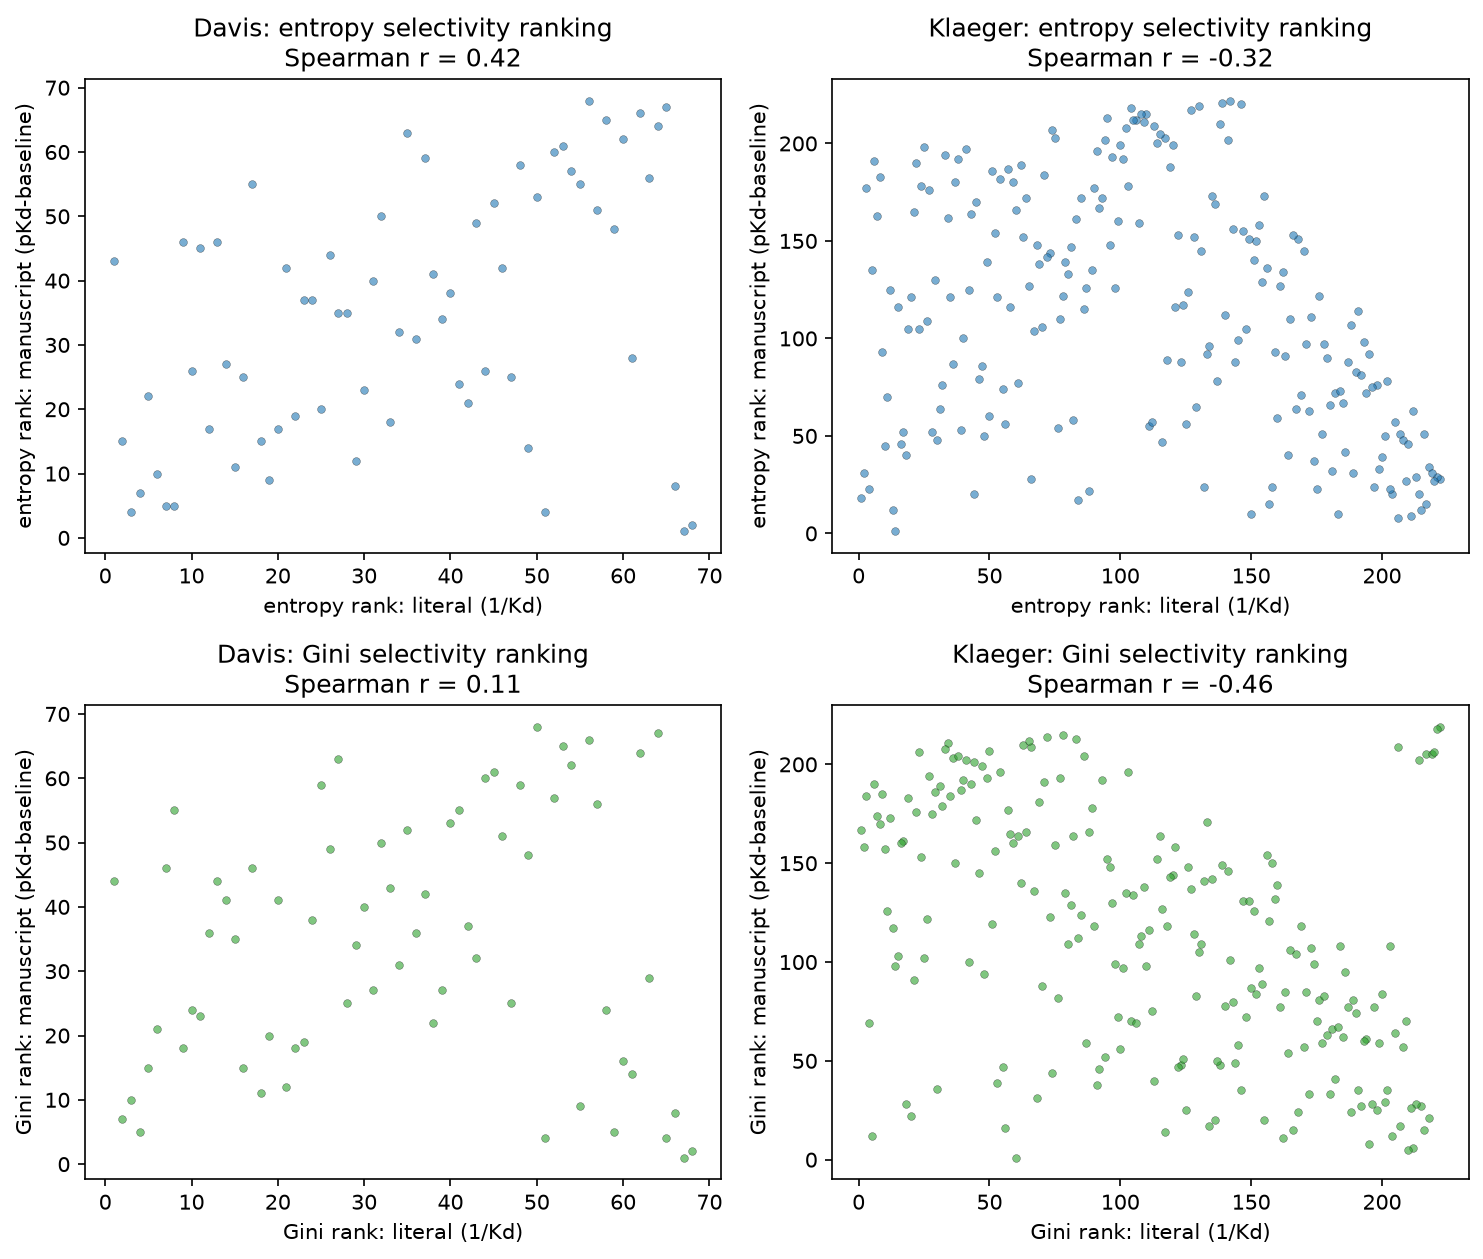
\includegraphics[width=\textwidth]{figures/metric_fidelity}
  \caption{Operationalization sensitivity of the entropy and Gini coefficient.
           For each dataset, the compound selectivity ranking computed in a form
           close to the original publication (association-constant weighting) is
           plotted against the baseline-subtracted log-affinity form used in the
           main text. Top row: selectivity entropy; bottom row: Gini coefficient.
           The two operationalizations of the same named metric differ
           substantially, and the entropy ranking even reverses on Klaeger,
           confirming that the operationalization of a named metric is a
           source of the definitional instability.}
  \label{fig:fidelity}
\end{figure}

\subsection{Rank Stability Analysis}
\label{sec:methods:stability}

For each definition and each parameter value, compounds were ranked from most
selective (rank 1) to least selective (rank $n$, where $n$ is the number of
compounds in the dataset).
Ties were broken by average rank.
This yielded 30 rank vectors per dataset for Davis, Klaeger, and Metz (11 for
the S-score, 7 for entropy, 7 for Gini, and 5 for ratio), and 28 for
Anastassiadis, whose coarser native percent-inhibition scale supports only 9
S-score threshold values rather than 11.

For each compound, rank instability was quantified as the standard deviation
of its rank across all configurations for that dataset (overall instability)
and separately
across parameter configurations within each definition family (within-family
instability).
Cross-definition-family agreement was assessed using Spearman rank correlation
between the median rank vectors of each definition family.
The median was taken across parameter values within each family, rather than
the mean, because the
median is less sensitive to the inclusion or exclusion of outliers than the mean.

Associations between rank instability and binding profile features were
assessed using Spearman correlation, restricted to the Klaeger and Davis
datasets. These are the two datasets on a $\mathrm{p}K_d$ scale, so the same
activity threshold and affinity-based features apply directly, allowing the
predictor structure to be checked for replication across a second dataset.
Profile features computed for each compound included: the number of active
kinases ($\mathrm{p}K_d > 6$), the gap between the top and second-ranked
affinities, the standard deviation and range of active affinities, and the
absolute affinity of the second-ranked target.
All correlations are reported with two-tailed $p$-values. Significance
thresholds of $p < 0.05$, $p < 0.01$, and $p < 0.001$ are denoted *, **, and
*** respectively.
Analyses were performed in Python 3.10 using NumPy, pandas, and
SciPy.\cite{NumPy,pandas,SciPy}
A secondary analysis relating selectivity rankings to clinical adverse-event
outcomes (FAERS report rates and FDA-label discontinuation rates for the
FDA-approved Klaeger compounds) is summarized in the Limitations section.
The analysis code and full per-definition results are available in the code
repository (see Data and Software Availability).

\section{Results}
\label{sec:results}

\subsection{Selectivity Definitions Cluster into Two Families}
\label{sec:results:families}

Across 30 parameter configurations (11 S-score thresholds, 7 entropy
baselines, 7 Gini baselines, 5 ratio off-target indices), compound rankings
were computed for all drugs in both datasets.
Spearman correlations between the median ranking of each definition family
reveal a consistent two-cluster structure (Table~\ref{tab:correlations}).
On the Davis dataset, S-score, entropy, and Gini are mutually correlated
($r = 0.95$--$0.999$), while ratio correlates substantially less with each
($r = 0.34$--$0.46$).
On the larger Klaeger dataset, the same structure is preserved but with lower
within-cluster correlations ($r = 0.72$--$0.90$), reflecting greater
diversity of binding profiles among the 222 clinical compounds.
The ratio definition is the consistent outlier in both datasets, with
cross-family correlations of $r = 0.22$--$0.62$.

\begin{table}[h]
  \centering
  \caption{Spearman correlations between median rankings by definition family.
           Upper triangle: Davis ($n=68$). Lower triangle: Klaeger ($n=222$).}
  \label{tab:correlations}
  \begin{tabular}{lcccc}
    \toprule
                & S-score & Entropy & Gini  & Ratio \\
    \midrule
    S-score     & ---     & 0.946   & 0.952 & 0.456 \\
    Entropy     & 0.901   & ---     & 0.999 & 0.343 \\
    Gini        & 0.722   & 0.866   & ---   & 0.343 \\
    Ratio       & 0.223   & 0.483   & 0.616 & ---   \\
    \bottomrule
  \end{tabular}
\end{table}

This two-family structure reflects a fundamental difference in what the
definitions measure.
The S-score, entropy, and Gini all quantify the concentration of activity
across the full kinase panel. They differ in functional form but respond to
the same underlying property of the binding profile.
The ratio definition, by contrast, quantifies the gap between the primary
target and a specific off-target, ignoring the remainder of the binding
profile entirely.
A compound that strongly inhibits one kinase and moderately inhibits twenty
others will be ranked as highly selective by ratio (large gap to the
second target) but as moderately promiscuous by entropy and Gini
(activity distributed across many targets).

\subsection{The Two-Family Structure Replicates Across Assay Technologies}
\label{sec:results:replication}

The Davis and Klaeger pattern of Table~\ref{tab:correlations} extends to the two
further datasets, across three assay technologies and both readout types
(Figure~\ref{fig:crossdataset}).
In all four, the S-score, entropy, and Gini remain mutually correlated
(within-family Spearman $r = 0.72$--$0.999$) while the ratio definition is the
consistent outlier. Its correlation with the distribution-based family is
$0.49$--$0.56$ on the Anastassiadis functional-activity dataset and only
$0.14$--$0.19$ on the Metz $\mathrm{p}K_i$ dataset.
The degree of separation varies with the assay, but in every case the ratio
definition measures something the distribution-based definitions do not.

The instability findings also replicate.
Compounds with no active kinases (Type~1, below) are markedly more rank-unstable
than active compounds wherever such compounds exist: mean rank
$\sigma = 36.8$ vs.\ $21.7$ on Anastassiadis and $178.5$ vs.\ $108.1$ on Metz,
matching the $72.9$ vs.\ $31.3$ contrast on Klaeger (Davis contains no
zero-active compounds).
Within the distribution-based family, the number of active kinases negatively
predicts entropy instability in every dataset ($r = -0.28$ to $-0.43$), and the
top$_1$--top$_2$ affinity gap predicts ratio instability on Davis, Klaeger, and
Metz ($r = -0.44$, $-0.34$, $-0.27$; all $p < 0.001$), as detailed below.

\begin{figure}[h]
  \centering
  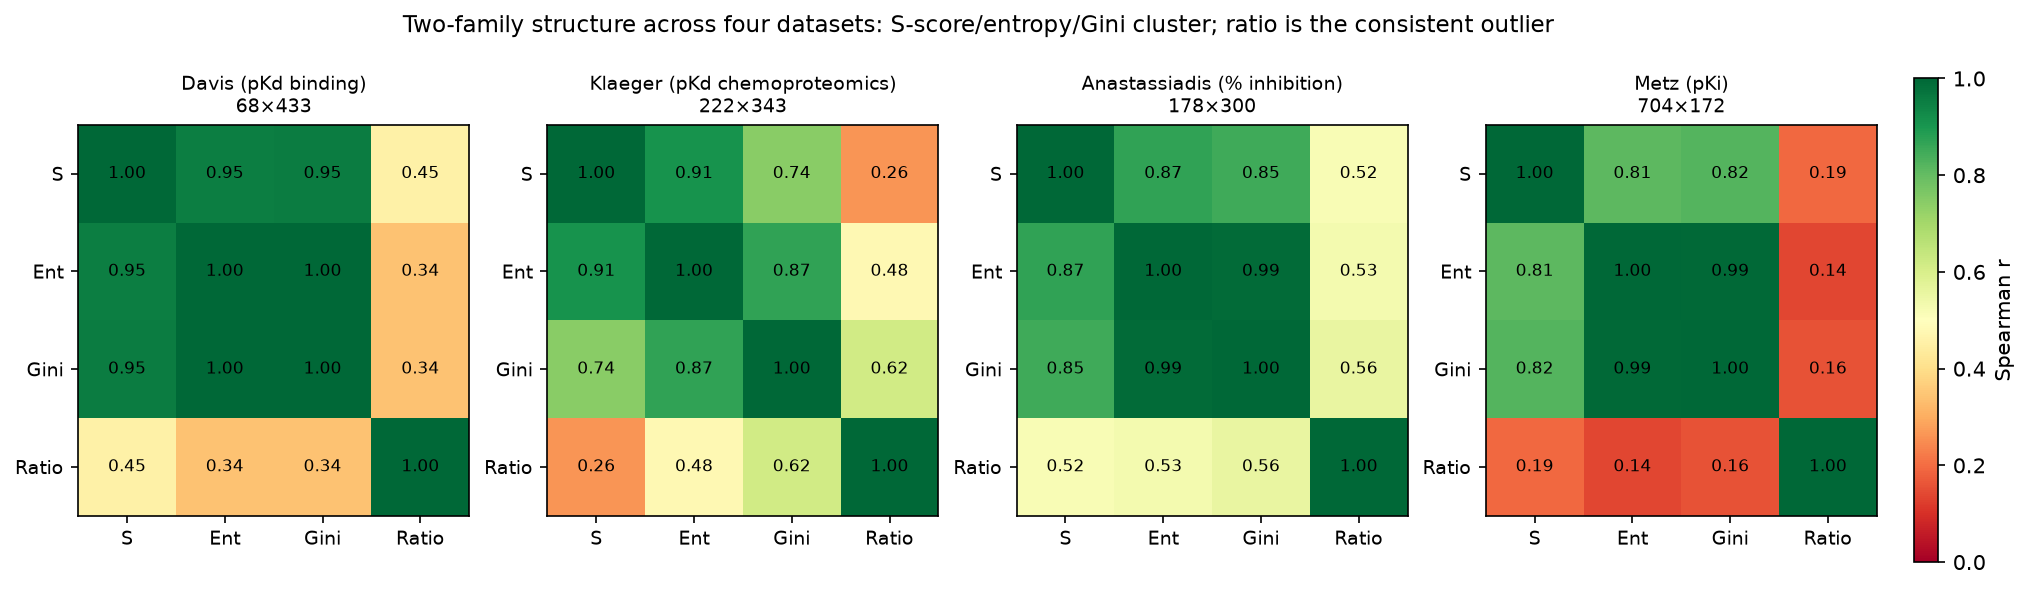
\includegraphics[width=\textwidth]{figures/cross_dataset_correlations}
  \caption{Spearman correlations between the median rankings of the
           four selectivity definitions, computed independently on each of the
           four datasets (compound $\times$ kinase panel sizes shown).
           In every dataset the S-score (S), entropy (Ent), and Gini cluster
           together while the ratio is the consistent outlier (the ratio row
           and column are the least green throughout), confirming the
           two-family structure across competition-binding, chemoproteomic, and
           functional-activity assays.}
  \label{fig:crossdataset}
\end{figure}

\subsection{Rank Instability Is Structured and Predictable}

\begin{figure}[h]
  \centering
  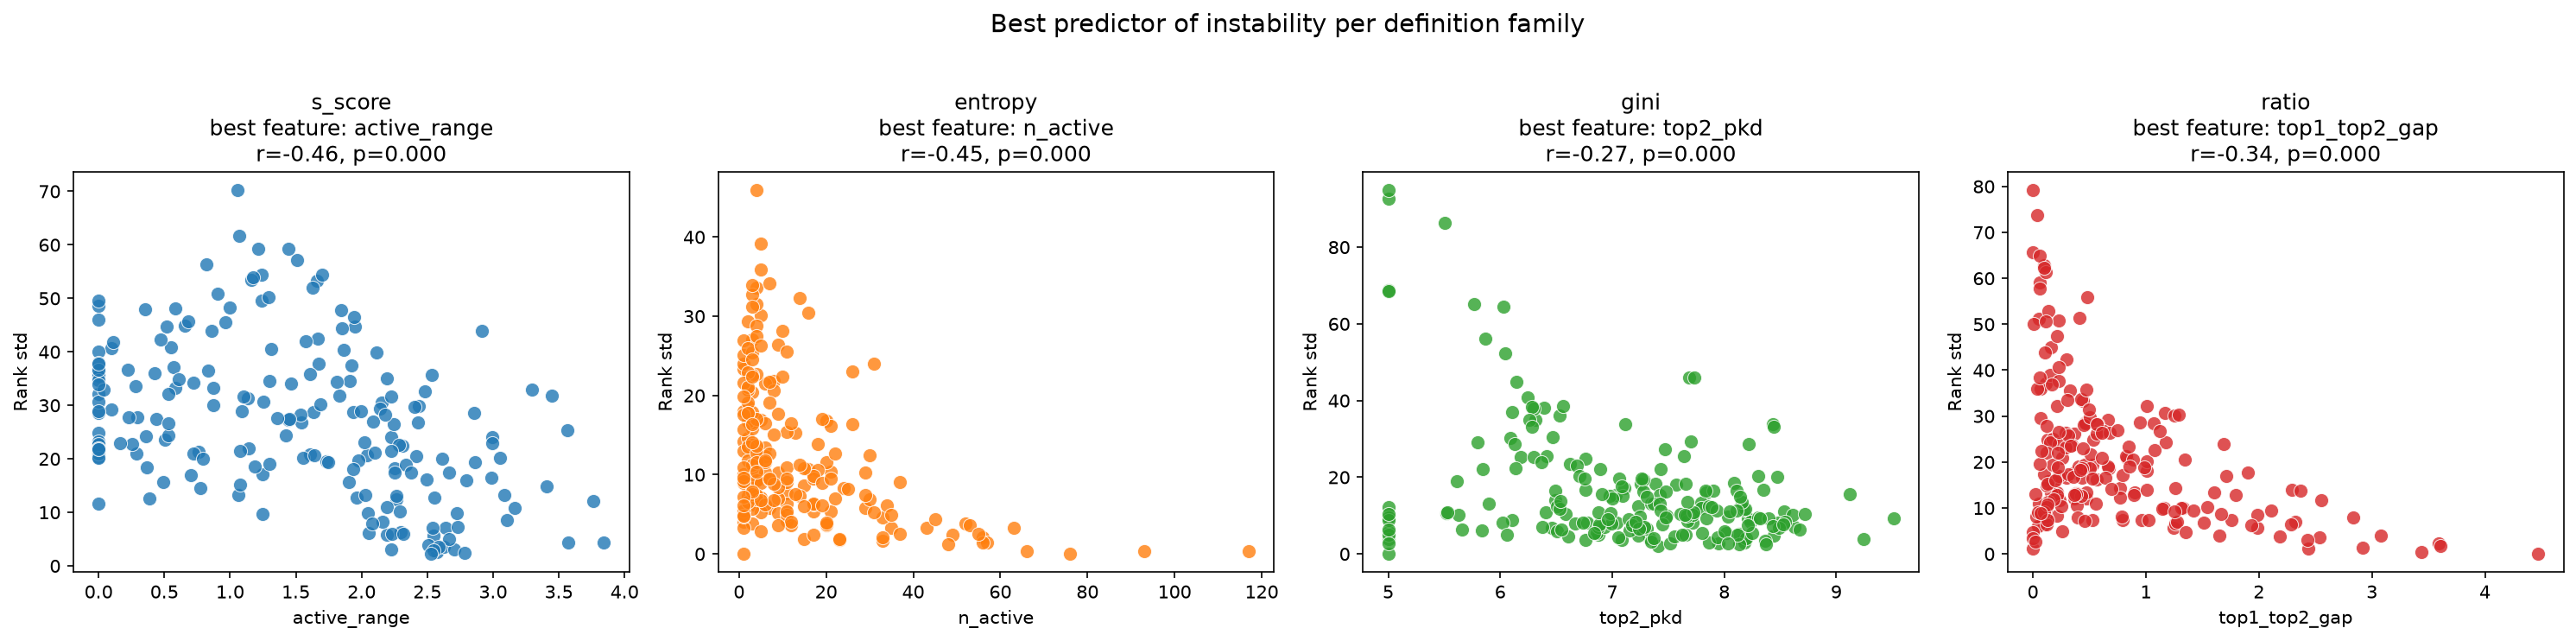
\includegraphics[width=0.85\textwidth]{figures/instability_by_family}
  \caption{Best predictor of rank instability within each definition family
           (Klaeger dataset, active compounds, $n=206$).
           Ratio instability is best predicted by the top$_1$--top$_2$ affinity gap;
           entropy, Gini, and S-score instability are best predicted by features
           of the active affinity distribution.}
  \label{fig:instability}
\end{figure}

\label{sec:results:instability}

Overall rank instability (measured as the standard deviation of a
compound's rank across all 30 configurations) varies substantially across
compounds (Klaeger: mean $\sigma = 34.3$, range $7.0$--$90.7$;
Davis: mean $\sigma = 8.5$, range $1.8$--$19.3$).
Instability is not uniformly distributed: within each definition family,
specific binding profile features predict which compounds receive unstable
rankings (Table~\ref{tab:predictors}).

Within the ratio family, the gap between the top and second-ranked affinities
(top$_1$--top$_2$ gap) is the strongest predictor of instability
(Figure~\ref{fig:instability})
($r = -0.444$, $p < 0.001$ on Davis, and $r = -0.341$, $p < 0.001$ on Klaeger).
Compounds with near-identical affinities for their two best-bound kinases
receive highly variable ratio rankings because the choice of reference
off-target ($k = 1$ vs.\ $k = 2, \ldots, 5$) determines whether the compound
appears selective or promiscuous.

Within the entropy and Gini families, the number of active kinases
($\mathrm{p}K_d > 6$) negatively predicts instability
($r = -0.279$, $p < 0.05$ for entropy on Davis,
$r = -0.409$, $p < 0.001$ on Klaeger).
Compounds with many active kinases have well-defined broad profiles whose
entropy and Gini scores are stable across baseline choices, while compounds with few
active kinases are sensitive to the baseline because small changes can move
targets in or out of the active set, altering the distribution substantially.
The active affinity range is also a significant predictor for the S-score and
entropy on Klaeger ($r = -0.35$ and $-0.27$, both $p < 0.001$). Gini is not
significantly predicted by this feature ($r = -0.10$, $p = 0.15$). It is consistent with the interpretation that heterogeneous
profiles (whose affinities span a wide range) yield more reproducible rankings
across parameter choices than flat profiles (in which many near-equal affinities
reshuffle as the parameter changes).

Gini instability's strongest 
predictor in either dataset
($r = +0.346$, $p < 0.001$ on Klaeger) is skewness, exceeding every other feature--family
pairing in Table~\ref{tab:predictors} apart from the ratio's top$_1$--top$_2$
dependence. Unlike the other features above, it
targets what Gini measures directly, i.e. the shape of
the active-affinity distribution's inequality.
The positive sign of this correlation is consistent with right-skewed active
distributions being the least stable. Most active kinases bound only modestly
above threshold, with one (or a few)
much more potent outliers, concentrating mass near the baseline boundary.
A small shift in $\beta$ moves that mass in or out of the active set.
Left-skewed profiles (most active kinases tightly bound, few sitting near
threshold) are comparatively insensitive to that choice. As with active
affinity std/range above, the relationship does not replicate on Davis
($r = +0.043$, $p = 0.73$).

Unlike the other families, the S-score's instability is significantly predicted
by every profile-shape feature except the top$_1$--top$_2$ gap
(Table~\ref{tab:predictors}), and most strongly by the spread of active
affinities. Compounds whose active affinities cluster near the threshold gain or
lose panel hits under small shifts in $\tau$, whereas those with a wide affinity
range retain a stable hit count regardless of the exact cutoff.
This S-score pattern is specific to Klaeger, however, on Davis, no profile feature
significantly predicts S-score instability (all $|r| \le 0.16$;
Table~\ref{tab:predictors}, right). A possible explanation is that a threshold
count's instability is governed by where each assay's detection window falls
relative to the cutoff, and the two assays place
that window very differently: 3.6\% of the Klaeger matrix is active versus
17.9\% of Davis (Methods). 
The one predictor that replicates cleanly across both datasets is the
ratio family's dependence on the top$_1$--top$_2$ gap (above), which compares
two affinities directly rather than counting how many pass a cutoff. The entropy
dependence on the number of active kinases replicates in direction but more
weakly on the smaller Davis panel ($r = -0.409$ on Klaeger vs.\ $-0.279$ on
Davis). Gini shows the reverse pattern in strength, reaching significance on
Davis ($r = -0.300$) but not on Klaeger ($r = -0.093$).

\begin{table}[h]
  \centering
  \caption{Spearman correlations between binding profile features and
           within-family rank instability, on the Klaeger ($n=206$ active drugs)
           and Davis ($n=68$) datasets. Columns are the S-score (S), entropy (E),
           Gini (G), and ratio (R) families. The ratio family's dependence on the
           top$_1$--top$_2$ gap replicates strongly on both datasets. The
           S-score's dependence on the active-affinity spread does not (no feature
           is significant on Davis), and neither does Gini's dependence on
           active-affinity skew. Significance:
           * $p<0.05$, ** $p<0.01$, *** $p<0.001$.}
  \label{tab:predictors}
  \resizebox{\textwidth}{!}{%
  \begin{tabular}{lcccc@{\hskip 1.4em}cccc}
    \toprule
    & \multicolumn{4}{c}{Klaeger ($n=206$)} & \multicolumn{4}{c}{Davis ($n=68$)} \\
    \cmidrule(lr){2-5}\cmidrule(lr){6-9}
    Feature & S & E & G & R & S & E & G & R \\
    \midrule
    $n_\mathrm{active}$      & $-0.272^{***}$ & $-0.409^{***}$ & $-0.093$       & $-0.040$       & $-0.153$ & $-0.279^{*}$ & $-0.300^{*}$ & $+0.294^{*}$ \\
    top$_1$--top$_2$ gap     & $+0.039$       & $+0.082$       & $+0.031$       & $-0.341^{***}$ & $-0.079$ & $-0.007$     & $-0.029$     & $-0.444^{***}$ \\
    Active affinity std      & $-0.281^{***}$ & $-0.170^{*}$   & $-0.117$       & $-0.107$       & $+0.009$ & $-0.015$     & $+0.005$     & $+0.040$ \\
    Active affinity range    & $-0.354^{***}$ & $-0.273^{***}$ & $-0.102$       & $-0.116$       & $+0.011$ & $-0.111$     & $-0.098$     & $+0.134$ \\
    top$_2$ $\mathrm{p}K_d$  & $-0.314^{***}$ & $-0.234^{***}$ & $-0.192^{**}$  & $+0.186^{**}$  & $-0.055$ & $-0.203$     & $-0.187$     & $+0.296^{*}$ \\
    Active affinity skew     & $-0.162^{*}$   & $-0.045$       & $+0.346^{***}$ & $-0.108$       & $+0.026$ & $+0.066$     & $+0.043$     & $+0.069$ \\
    \bottomrule
  \end{tabular}%
  }
\end{table}

Five additional candidates features were tested:
two concentration measures from industrial-organization
economics ((1) the top-target concentration ratio (CR$_1$) and (2) the
Herfindahl--Hirschman Index (HHI)). These were sourced from the same 
field as the Gini coefficient \cite{Graczyk2010}. We also tested
(3) the raw
primary-target affinity (top$_1$ $\mathrm{p}K_d$), (4) a near-tie count
generalizing the top$_1$--top$_2$ gap, and (5) the active-affinity coefficient of
variation. CR$_1$ and HHI turned out to be near-collinear with
$n_\mathrm{active}$, which is already in the table ($r = -0.98$ to $-0.99$ and $-0.998$,
respectively, on both datasets). The
remaining three were uniformly weaker predictors than the features already
included, in every family and both datasets (full numbers in the code
repository).

\subsection{Three Mechanistically Distinct Sources of Instability}

\begin{figure}[h]
  \centering
  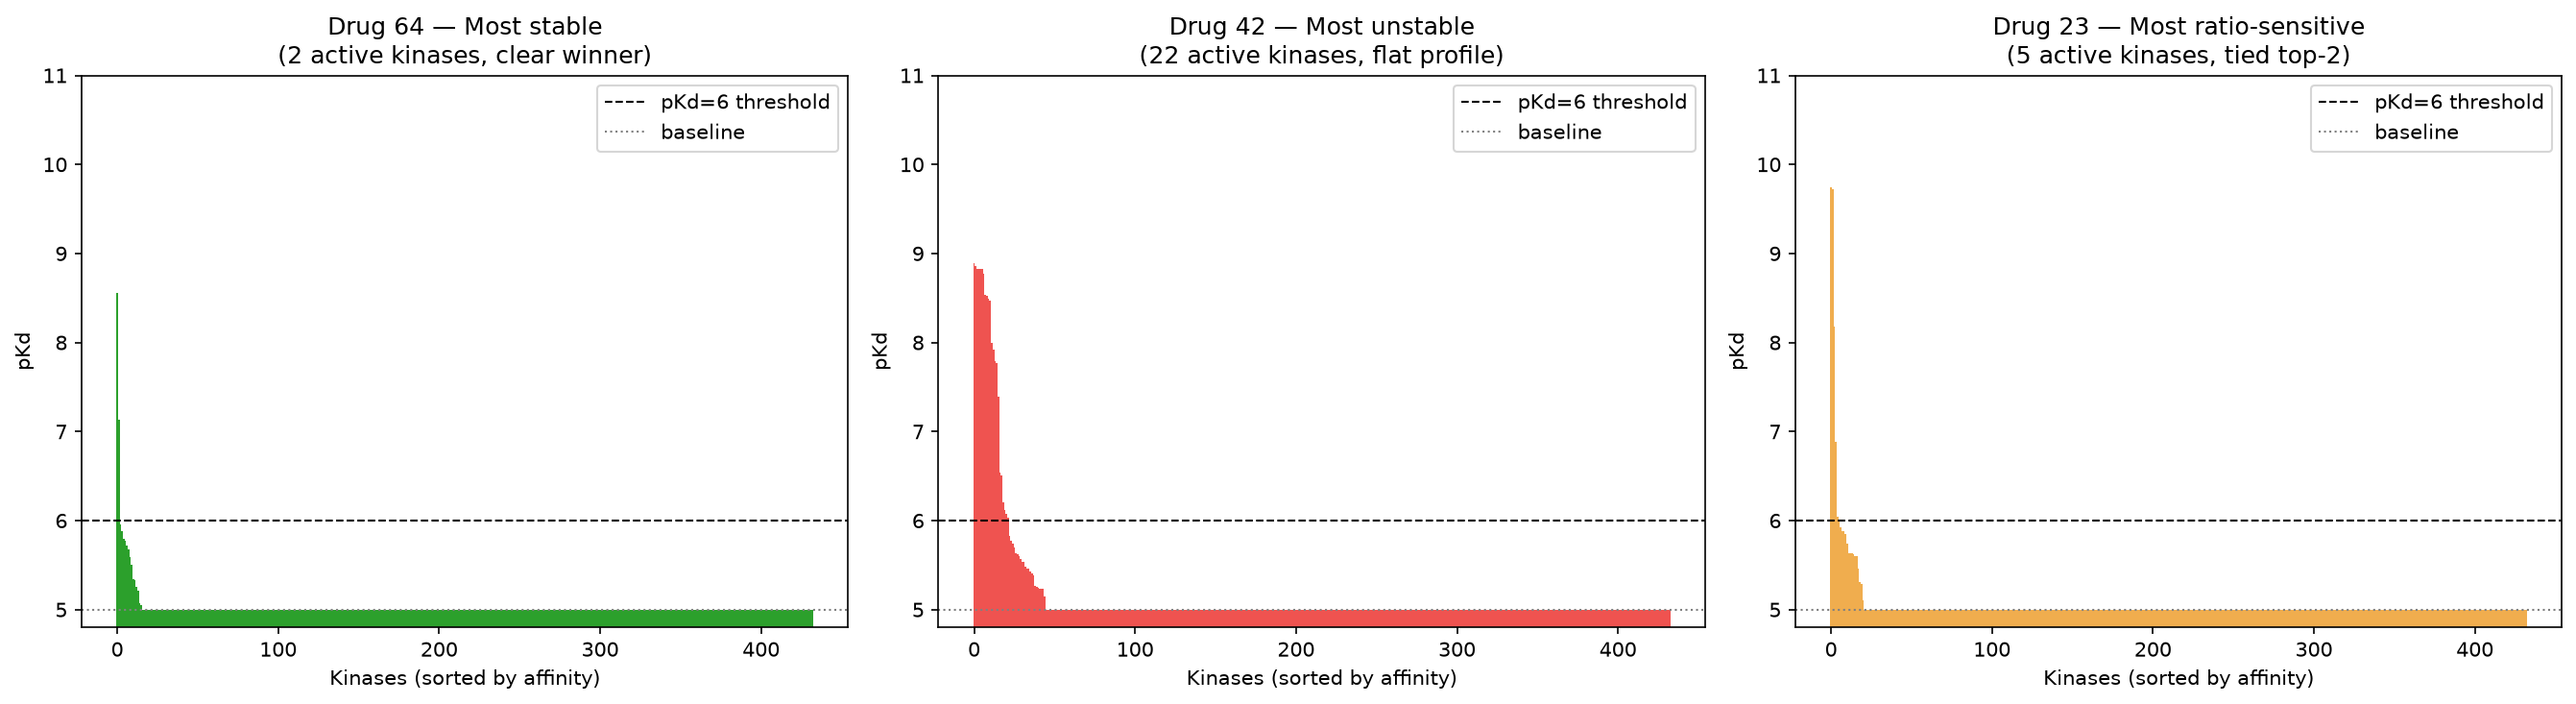
\includegraphics[width=0.85\textwidth]{figures/binding_profiles}
  \caption{Representative binding profiles illustrating the three instability types.
           Left: Drug~64 (Davis), most stable ($\sigma = 1.8$), two active kinases.
           Center: Drug~42 (Davis), most unstable ($\sigma = 19.3$), 22 active kinases
           with no dominant target.
           Right: Drug~23 (Davis), most ratio-sensitive, five active kinases
           including two near-tied top targets ($\Delta\mathrm{p}K_d = 0.023$).
           Dashed line: $\mathrm{p}K_d = 6$ activity threshold;
           dotted line: $\mathrm{p}K_d = 5$ assay floor.}
  \label{fig:profiles}
\end{figure}

\label{sec:results:taxonomy}

Examination of the most and least unstable compounds in the Klaeger dataset
reveals three structurally distinct sources of rank instability
(Figure~\ref{fig:profiles}), each
implicating a different aspect of how the definitions are constructed.

\textbf{Type~1: Zero-active compounds.}
The five most unstable Klaeger compounds (AZD-8055, BMS-911543, Vatalanib,
Filgotinib, ARRY-380; rank $\sigma > 76$) all have zero active kinases at the
$\mathrm{p}K_d > 6$ threshold.
These compounds have no meaningful binding to any profiled kinase at
sub-micromolar affinity, yet all four definitions still assign them numerical
selectivity scores based on the detection floor values.
The resulting rankings are arbitrary: different parameterizations produce
different orderings of compounds that are, in practice,
indistinguishable from one another.
Mean rank instability for zero-active compounds is $\sigma \approx 73$,
compared with $\sigma \approx 31$ for compounds with at least one active
kinase ($p < 0.001$, Mann--Whitney $U$ test).
Davis has no such compounds at all: every Davis compound
has at least one active kinase, consistent with Davis's fixed-concentration
screening design, which reports a $K_d$ only when activity is first detected
at 10~$\mu$M. The same zero-active instability contrast reported here for
Klaeger also holds on the two further datasets in
Section~\ref{sec:results:replication}.

\textbf{Type~2: Near-tied top targets.}
When an active compound's two best-bound kinases have near-identical affinities, the
ratio is highly sensitive to which is designated the primary target and which
the reference off-target, because a small parameter change can swap their roles
(the top$_1$--top$_2$ gap is the strongest predictor of ratio instability, above).
Drug~23 in the Davis dataset (top$_1$--top$_2$ gap $= 0.023$~pKd units) is the
extreme case: its two best-bound kinases are essentially indistinguishable, so
it receives maximally unstable ratio rankings.

\textbf{Type~3: Broad profiles with a dominant primary target.}
The largest entropy-ratio disagreements in the Klaeger dataset arise for
compounds with high $n_\mathrm{active}$ and a large top$_1$--top$_2$ gap
(e.g.\ Dovitinib: $n_\mathrm{active} = 26$, gap $= 1.935$;
BMS-690514: $n_\mathrm{active} = 20$, gap $= 1.985$).
These compounds have one clearly dominant target but also bind many kinases at
moderate affinity.
The ratio definition scores them as highly selective (large gap between primary
and secondary target), while the entropy and Gini definitions score them as
moderately promiscuous (activity spread across many targets).
Neither characterization is incorrect, as they reflect genuinely different
questions about selectivity. 

Conversely, the most stable compounds in both datasets (e.g.\ XL-228,
$\sigma = 7.0$; PF-03814735, $\sigma = 7.8$) are highly promiscuous, with
55--57 active kinases.
When a compound binds nearly the entire profiled kinome, all definitions rank
it as non-selective regardless of parameterization, producing low instability.

\subsection{Panel Size Dependence of Selectivity Rankings}
\label{sec:results:panelsize}

To assess the stability of selectivity rankings as a function of kinase panel
size, we performed a subsampling analysis on the two datasets with genuine
sparse kinase coverage: Klaeger (343 kinases, chemoproteomic dose--response
profiling) and Metz (172 kinases, a medicinal-chemistry campaign), in each of
which compounds were tested against only a subset of the panel.
The Davis and Anastassiadis datasets were not used for this analysis, because
both are dense complete-matrix screens (every compound tested against every
kinase by construction) rather than the sparse coverage of real profiling
panels. Subsampling their kinases would also change the apparent number of
active compounds in ways that confound the panel size effect with the
zero-active instability characterized in the instability taxonomy above.

For each panel size (Klaeger $p \in \{50, 80, \ldots, 320, 343\}$; Metz
$p \in \{50, 80, \ldots, 170, 172\}$), we drew 50 random subsets of $p$ kinases
from the full panel, computed each selectivity definition on the subpanel, and
measured agreement with the full-panel ranking using Spearman correlation.
We call a panel size ``recovering'' the full-panel ranking once this mean
correlation exceeds $0.90$, adopting the same numerical bar reliability
conventionally sufficient to call a measurement ``excellent'' \cite{Koo2016}. 
Altering the choice of correlation cutoff changes the reported $p^*$ values,
however, the
ratio definition remains the slowest to recover and the Gini coefficient the
second-slowest for any bar between $0.80$ and $0.95$. Only the relative order
of entropy and the S-score is bar-dependent within this range (full numbers
in the code repository).

On Klaeger, the four definitions differ substantially in their panel size
requirements (Figure~\ref{fig:panelsize}).
Selectivity entropy and the S-score both reach mean $r = 0.90$ against the
full-panel ranking at approximately 110 kinases.
The Gini coefficient requires approximately 290 kinases to reach the same
threshold.
The ratio definition does not reach $r = 0.90$ at any subpanel size short of
the full panel: it achieves only $r = 0.888$ even at 320 kinases, just 23
below the full panel of 343, and attains $r = 0.90$ only on the complete panel.

This result has a direct practical implication.
Standard commercial kinase selectivity panels typically profile 50--100
kinases.\cite{Bosc2017}
At these panel sizes, entropy- and S-score-based rankings are reasonably
stable ($r \approx 0.76$--$0.85$), but Gini and ratio rankings are effectively
uncorrelated with what would be obtained on a full kinome panel
($r < 0.14$ for Gini, $r < 0.00$ for ratio at $p = 50$).
Ratio rankings in particular are unreliable at any panel size commonly used
in practice, because the identity of the reference off-target ($k$-th ranked
kinase) changes substantially as panel composition changes.

To test whether these patterns generalize beyond a single assay, we repeated the
analysis on Metz (172 kinases; Figure~\ref{fig:panelsize}, right). The ordering
of the definitions by panel-size requirement is preserved. The distribution-based
definitions recover the full-panel ranking from a small fraction of the panel
(S-score at approximately 50 kinases, entropy and Gini at approximately 80),
while the ratio again lags, reaching $r = 0.90$ only at 170 of the 172 kinases.
We note that the ratio's poor recoverability is universal, holding
on both sparse datasets, which strengthens the case that it measures a distinct,
panel-composition-dependent property. We also note that the Gini coefficient is the one
measure whose recoverability is dataset-specific. It is slow on Klaeger ($p^* = 290$),
but fast on Metz ($p^* = 80$), so its poor behavior on Klaeger should not be read
as a general property. Entropy and the S-score are fast on both.

\begin{figure}[h]
  \centering
  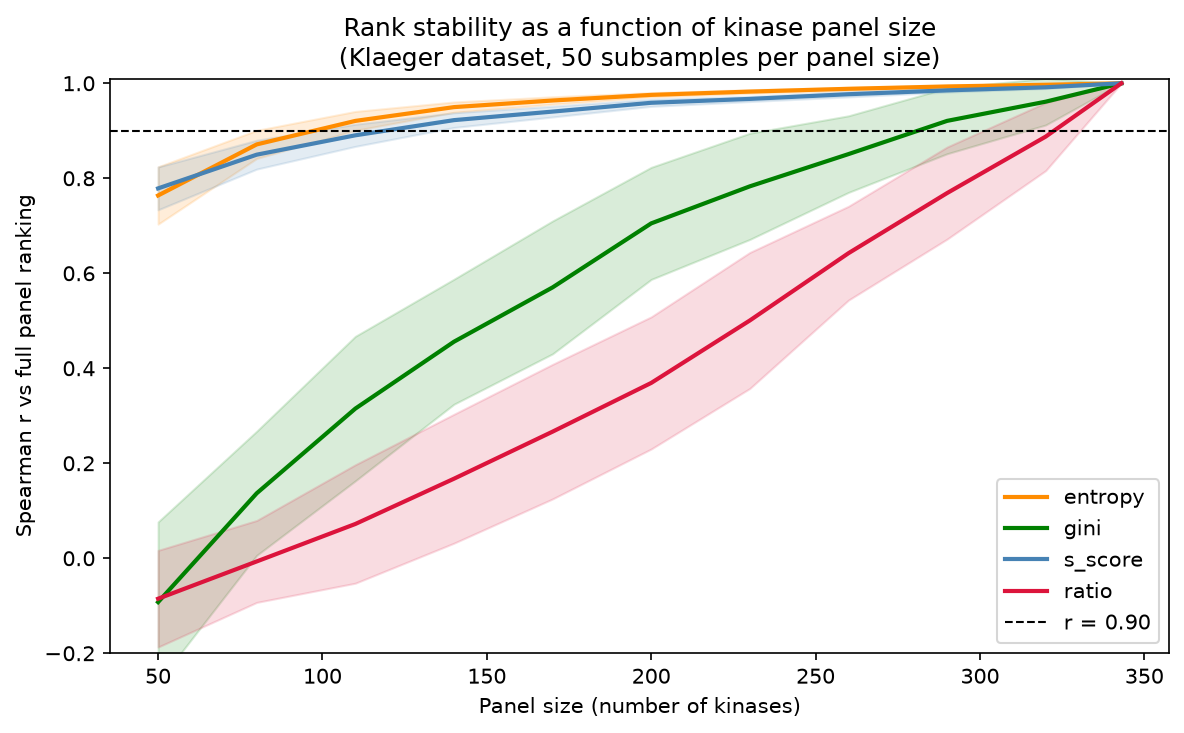
\includegraphics[width=\textwidth]{figures/panel_size_stability}
  \caption{Mean Spearman correlation between rankings computed on random kinase
           subpanels and rankings on the full panel, as a function of subpanel
           size, for the two sparse-coverage datasets: Klaeger (left, 343 kinases)
           and Metz (right, 172 kinases).
           Shaded bands indicate $\pm 1$ standard deviation across 50 subsamples;
           the dashed line marks $r = 0.90$.}
  \label{fig:panelsize}
\end{figure}

\section{Required Properties for a Well-Formed Selectivity Measure}
\label{sec:desiderata}

The empirical findings of the Results section motivate four properties that any
well-formed kinase inhibitor selectivity measure should satisfy.
Each property is stated below together with the observed failure mode that
motivates it.

Let $\mathbf{x} = (x_1, \ldots, x_N) \in \mathbb{R}^N$ denote a compound's
binding profile across $N$ kinases, where $x_i = \mathrm{p}K_{d,i}$.
$N$ is the size of the profiling panel, which varies
across compounds within a dataset (Anastassiadis, Metz) and across datasets
(Davis: $N=433$; Klaeger: $N=343$).
A selectivity measure is a function $f : \mathbb{R}^N \to \mathbb{R}$, where
higher values indicate greater selectivity, defined for every panel size $N$.
A selectivity ranking over a set of compounds is induced by ordering their
$f$-scores.

\paragraph{D1: Reliability threshold.}
There exists a threshold $\tau^* > 0$ such that $f(\mathbf{x})$ is undefined,
or explicitly flagged as unreliable, when $\max_i x_i \leq \tau^*$.

\textit{Motivation.}
Compounds with no detected binding above the assay detection floor receive
arbitrary selectivity scores under all four definitions studied here, producing
rank instability with mean $\sigma \approx 73$ compared with $\sigma \approx
31$ for active compounds (Type~1 instability, above; Figure~\ref{fig:failure_modes}, left).
A compound that does not bind cannot be
meaningfully ranked relative to compounds that do.
No existing definition incorporates an explicit reliability condition.
In fact, both
the S-score and selectivity entropy assign scores to compounds with no
sub-micromolar binding, treating detection floor values as informative.

\paragraph{D2: Bounded gap sensitivity.}
For any compound profile $\mathbf{x}$ satisfying D1, a small perturbation to
the identity of the reference off-target should produce a bounded change in
$f(\mathbf{x})$.
Formally, if $f$ depends on the $k$-th ranked affinity $x_{(k)}$, then there
should exist a function $g$ with $g(0) = 0$ such that
$|f(\mathbf{x}; k) - f(\mathbf{x}; k+1)| \le g(x_{(k)} - x_{(k+1)})$. This 
inequality states that ``as the gap
between the two ranked affinities shrinks to zero, the score's dependence on
which one is chosen as the reference off-target must shrink to zero as well''.

\textit{Motivation.}
Ratio-based definitions violate this property when $x_{(1)} \approx x_{(2)}$.
A compound with near-identical affinities for its top two kinases receives a
large ratio score when $k=1$ (the gap to the next off-target may be large) but
a near-zero score when $k=2$ (the gap between the tied targets is negligible).
This produces the Type~2 instability identified in
the instability taxonomy above, where top$_1$--top$_2$ gap is the
strongest predictor of ratio instability ($r = -0.341$, $p < 0.001$).
Entropy and Gini satisfy D2 vacuously. 
Neither scores a specific ranked affinity $x_{(k)}$, so the \emph{if} 
condition of D2's formal statement
(``if $f$ depends on the $k$-th ranked affinity, then \ldots'') is never
satisfied.
However, they also satisfy the intent of D2. 
That is, both are symmetric, continuous functions of
the full normalized profile, so swapping two exactly tied affinities leaves the
score unchanged, and a near-tie changes it only by a vanishing amount.
The S-score also has no $k$-th ranked term, but it is not continuous in the
same way: it counts kinases against a fixed threshold $\tau$, so whichever
kinase's affinity happens to sit nearest $\tau$ plays the role of a reference
off-target, and an infinitesimal perturbation that moves that affinity across
$\tau$ changes the score by a full $1/N$. This is a bounded, single-kinase
version of the same instability, smaller in magnitude than the ratio's
unbounded swing but not the vanishing sensitivity entropy and Gini show, which
is why it is graded $\sim$ rather than $\checkmark$ in
Table~\ref{tab:desiderata}.

\paragraph{D3: Distributional consistency.}
The ranking induced by $f$ should be stable under small perturbations to the
activity baseline $\beta$ used to define the active binding distribution.
Formally, for any two compounds $\mathbf{x}, \mathbf{y}$ and any
$\epsilon > 0$, there exists $\delta > 0$ such that if $|\beta_1 - \beta_2|
< \delta$ then the ranking of $\mathbf{x}$ relative to $\mathbf{y}$ under
$f(\cdot; \beta_1)$ agrees with that under $f(\cdot; \beta_2)$.

\textit{Motivation.}
The entropy and Gini definitions are parameterized by a baseline $\beta$ that
determines which affinities contribute to the binding distribution.
Compounds with few active kinases are sensitive to this choice because small
changes in $\beta$ can move individual kinases in or out of the active set,
substantially altering the distribution.
The negative correlation between $n_\mathrm{active}$ and entropy
instability ($r = -0.409$ on Klaeger, $p < 0.001$; weaker for Gini, see
Table~\ref{tab:predictors}) reflects this sensitivity
(Figure~\ref{fig:failure_modes}, right).
D3 requires that the ranking be robust to the choice of $\beta$ within a
reasonable neighborhood, which existing implementations do not guarantee.
The ratio $R(k)$ compares two specific ranked
affinities directly, so there is no $\beta$ for D3 to perturb. It therefore
has no activity baseline at all.
Unlike D2, D3's formal statement is not phrased as a conditional. Instead, it
presupposes a baseline $\beta$. Where that presupposition fails, as for
the ratio, the property holds vacuously. 
This is why the ratio is graded
$\checkmark$ for D3 in Table~\ref{tab:desiderata}.

The S-score's threshold $\tau$ plays the same
active/inactive gating role as $\beta$.
Its instability under $\tau$ is, however,
weaker and less consistent than entropy and Gini's under $\beta$. This instability is
predicted by every profile-shape feature except the top$_1$--top$_2$ gap on
Klaeger, but by none of them on Davis (all $|r| \le 0.16$;
Table~\ref{tab:predictors}). The entropy's $n_\mathrm{active}$
dependence, on the other hand, replicates on both datasets. 
This inconsistent sensitivity is why the S-score is
graded $\sim$ rather than $\times$ or $\checkmark$.

\paragraph{D4: Monotonicity under weak off-target addition.}
If compound $\mathbf{x}$ has a weak additional binding interaction added, i.e.
if $\mathbf{x}' = (x_1, \ldots, x_N, x_{N+1})$ where $x_{N+1} \leq
\tau^*$, then $f(\mathbf{x}') \leq f(\mathbf{x})$.
Adding a sub-threshold binding interaction should not increase a compound's
selectivity score.

\textit{Motivation.}
The S-score and the Gini coefficient violate this property.
Adding a kinase that the compound does not meaningfully bind increases the panel
size without adding activity. This lowers the S-score's fraction of hit kinases
and raises the Gini coefficient's inequality, in both cases inflating the
apparent selectivity.
A compound can therefore be made to look more selective simply by profiling it
against more inactive kinases. This is a serious problem when panels differ in size or
composition across experiments, as between Davis and Klaeger.
The entropy and the ratio satisfy D4. This can be explained by 
the fact that a sub-threshold target adds negligible
weight to the entropy's normalized distribution and falls at or below the
ratio's reference off-target, so neither score increases.

\bigskip
Table~\ref{tab:desiderata} summarizes which definitions satisfy each property.
No existing definition satisfies all four simultaneously, but the candidate measure
introduced next does.

\begin{table}[h]
  \centering
  \caption{Satisfaction of the four required properties by existing selectivity
           definitions and by the candidate measure introduced below.
           $\checkmark$: satisfied (by construction, or verified empirically for
           the candidate).
           $\sim$: partially satisfied or satisfied under additional assumptions.
           $\times$: violated in general.}
  \label{tab:desiderata}
  \begin{tabular}{lccccc}
    \toprule
    Property & S-score & Entropy & Gini & Ratio & Candidate \\
    \midrule
    D1 (reliability threshold)        & $\times$ & $\times$     & $\times$     & $\times$     & $\checkmark$ \\
    D2 (bounded gap sensitivity)      & $\sim$   & $\checkmark$ & $\checkmark$ & $\times$     & $\checkmark$ \\
    D3 (distributional consistency)   & $\sim$   & $\times$     & $\times$     & $\checkmark$ & $\checkmark$ \\
    D4 (monotonicity, weak off-target)& $\times$ & $\checkmark$ & $\times$     & $\checkmark$ & $\checkmark$ \\
    \bottomrule
  \end{tabular}
\end{table}

\subsection{A Candidate Measure}
\label{sec:candidate}

The four properties can indeed be satisfied, and the selectivity entropy is the
natural starting point.
The goal is not to outrank the entropy, but to repair the two failure modes
documented above (D1's arbitrary scores for non-binders and D3's
baseline-driven instability) without giving up what it already gets right.
Of the existing definitions it is the only one that already satisfies both D2 and
D4 (Table~\ref{tab:desiderata}). Because it scores the whole normalized profile
rather than a single pairwise gap, it neither privileges a reference off-target
(D2) nor rewards the addition of non-binders (D4).
It, however, fails D1 and D3. It fails D1 due to having no reliability gate.
The D3 failure comes from the hard active/inactive cutoff $\max(x_i - \beta, 0)$,
which ties the boundary between active and inactive kinases to the baseline
$\beta$. As $\beta$ moves, kinases enter or leave the active set and the ranking
shifts.
The cutoff plays two roles: it excludes non-binders, which keeps the measure
correctly oriented, and it sets the emphasis among the active kinases.
The candidate separates these roles. It excludes non-binders with a gate fixed at
the assay detection floor (a specified constant). 
It then applies a smooth softplus emphasis above the floor.
The ratio cannot be repaired this way, as it fails D2 by construction. The
S-score and Gini violate D4 by construction, as both are computed as a fraction or
rank-weighted sum over the full panel of size $N$. A sub-threshold addition
still shifts $N$ and moves the score. This differs from the entropy's
normalized weights, where a zero-weight addition drops out without changing the
score. The entropy is
therefore the one existing measure that can reach all four properties through
local changes.
The candidate differs from entropy in the following ways: 
(1) it adds the D1 reliability gate, (2) it fixes the
non-binder gate at the assay floor, and (3) it replaces the hard cutoff above the
floor with a smooth softplus emphasis.
For a profile $\mathbf{x}$ with $\max_i x_i > \tau^*$ (and undefined otherwise,
satisfying D1), define
\begin{equation}
  w_i = \mathbf{1}[x_i > x_0]\; T \log\!\big(1 + e^{(x_i - \beta)/T}\big), \qquad
  p_i = \frac{w_i}{\sum_j w_j}, \qquad
  f(\mathbf{x}) = \sum_i p_i \log_2 p_i,
\end{equation}
where $x_0$ is the fixed assay detection floor, $\beta$ is the emphasis baseline
(set to $x_0$ in the results below), and $T$ a smoothing width in
$\mathrm{p}K_d$ units.
The indicator gates out kinases at or below the floor, so non-binders carry no
weight. Without it, the non-binding kinases at the floor dominate
the profile and the score inverts, rising with the number of active kinases
($r = +0.94$ on Klaeger).
The score is the negative Shannon entropy of the smoothed, normalized profile, or,
equivalently, the negative logarithm of the effective number of targets the
compound binds.
The weight gate sits at the detection floor $x_0$, while the D1 reliability gate
sits at $\tau^* > x_0$. A kinase with affinity between $x_0$ and $\tau^*$ therefore
contributes to the binding distribution. However, a compound whose strongest binding
falls in that range is flagged unreliable by D1.

This measure satisfies all four properties.
D1 holds by the explicit reliability gate.
D2 holds because $f$ is a symmetric function of the full normalized profile and
references no particular off-target.
D3 holds because the candidate has no free activity baseline: the boundary
between active and inactive kinases is fixed at the assay detection floor $x_0$.
Entropy and Gini, as used in practice, leave
this baseline free, so their rankings move as it is varied (the
$n_\mathrm{active}$ instability correlation of Table~\ref{tab:predictors}).
Once $x_0$ is fixed, the sole free parameter left in the score is the softplus
emphasis baseline $\beta$, and the ranking is essentially invariant to it over
$[4.5, 6.5]$ (worst-case pairwise Spearman $\rho = 0.999$).
Moving the floor across the same range shifts the ranking sensitively
($\rho \approx -0.93$), as it does for any threshold-based activity
call, including the entropy's ($\rho \approx -0.95$).
D4 holds because the gated weight is zero at and below the floor and is monotone
above it, so adding a sub-threshold target never raises the score (verified for
$100\%$ of Klaeger compounds).
The orientation, D3, and D4 checks were repeated on the other three datasets.
The candidate stays correctly oriented and satisfies D3 and D4 on Davis,
Anastassiadis, and Metz, with orientation between selectivity and the
active-kinase count ranging from $-0.79$ to $-0.97$, D3 emphasis-robustness
$\rho \geq 0.99$, and D4 for $100\%$ of compounds in every dataset (full numbers
in the code repository).

\begin{figure}[h]
  \centering
  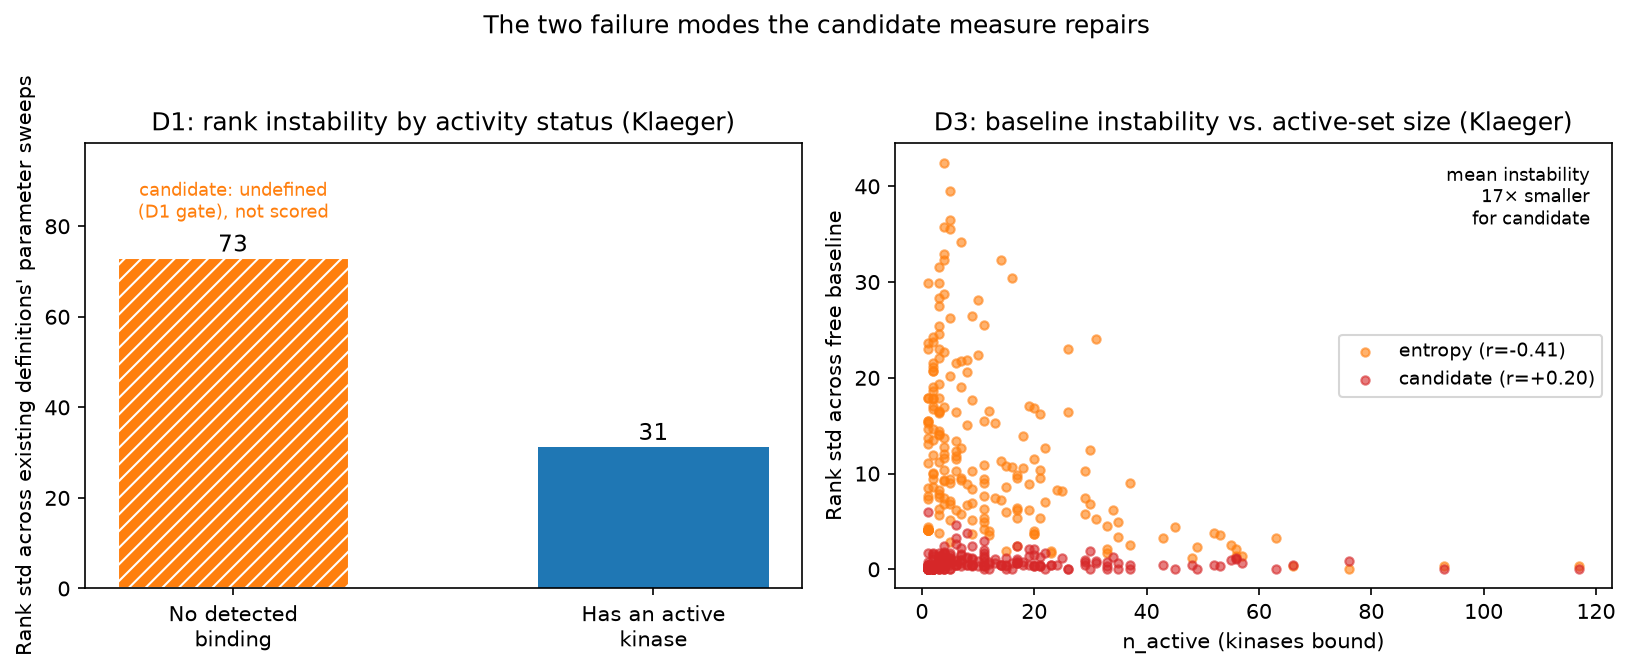
\includegraphics[width=\textwidth]{figures/failure_modes}
  \caption{The two failure modes the candidate measure repairs (Klaeger).
           \emph{Left (D1):} rank instability (std across the existing
           definitions' parameter sweeps) for compounds with no detected
           binding above the assay floor versus compounds with at least one
           active kinase; the candidate assigns the first group no score at
           all rather than an unstable one.
           \emph{Right (D3):} per-compound rank instability under the free
           activity baseline, against the number of active kinases, for the
           entropy and for the candidate. The entropy's instability grows as
           $n_\mathrm{active}$ shrinks; the candidate's stays near zero
           because it has no free activity baseline.}
  \label{fig:failure_modes}
\end{figure}

A usable measure must also be recoverable from realistic panels.
Applying the panel-size subsampling analysis above to the candidate (same grid,
50 random subpanels per size), the smallest panel reaching mean Spearman
$\rho > 0.90$ with the full-panel ranking is $p^* = 110$ kinases on Klaeger
(Figure~\ref{fig:candidate}) and $p^* = 80$ of 172 kinases on Metz, so it
converges quickly on both datasets.
On Klaeger, this matches the entropy and the S-score (all $p^* = 110$) and is
well ahead of the Gini ($290$) and the ratio ($343$, the full panel).
On Metz it again matches the entropy, but here the S-score converges faster
($p^* = 50$ vs.\ $80$).
Raw convergence speed is not by itself a useful criterion, however: the
S-score fails D1 and D4 outright (Table~\ref{tab:desiderata}), so a smaller
$p^*$ does not make it a viable alternative.
Matching the bare entropy's $p^*$ on both datasets, while adding the two
properties it lacks, shows that the D1 gate and the smooth emphasis do not
cost any convergence speed.

The candidate measure above is one member of a family of measures satisfying
D1--D4. Next, we consider three axes of variation within this family: the
reliability floor, the R\'enyi order, and the smoothing width $T$.
Replacing the fixed floor with a per-compound low-quantile
reference gives a shift-invariant variant.
It produces nearly the same ranking
on both datasets (Spearman $r \approx 1.00$), is equally robust to the choice of
quantile ($\rho \approx 1.00$ for D3), and continues to satisfy D4 exactly.

Generalizing the Shannon functional to any R\'enyi order $\alpha > 0$ gives
another way to vary the candidate solution:
$-H_\alpha(p) = \frac{1}{\alpha-1}\log_2 \sum_i p_i^\alpha$,
which recovers Shannon entropy as $\alpha \to 1$.
D1 holds for every $\alpha$ since the $x_0$ gate is applied before the entropy
is computed, independent of order. D2 and D3 hold by the same continuity and
symmetry arguments used for Shannon entropy, applied to $H_\alpha$ instead.
D4 holds because $p_i^\alpha = 0$ whenever $p_i = 0$, so a gated-out
coordinate cannot raise the score.
Although Spearman agreement with $\alpha = 1$ stays high ($0.997$--$1.000$ for
$\alpha \in \{0.5, 2, 3\}$ on both datasets), the orders are not redundant, and
$\alpha$ affects panel recoverability.
On Klaeger, $\alpha \in \{0.01, 0.25, 0.5, 0.75\}$ reaches $p^* = 80$,
ahead of the $\alpha = 1$ candidate's $p^* = 110$, while $\alpha \in \{2, 3\}$
falls to $p^* = 290$, matching the Gini. On Metz every order from $0.01$ to $3$
reaches $p^* = 80$, so this gap is specific to the sparser Klaeger panel.

This speed does not come from discarding information. The number of distinct
scores and the size of the largest tied group are identical across every order
tested, including $\alpha \to \infty$; the only tied compounds are those with at
most one active kinase, whose normalized profile is a point mass with zero
entropy regardless of order.
This reflects how each limit behaves under subsampling. As $\alpha \to 0$, the
score approaches a count of the active set, a quantity a random subpanel
estimates with low variance. As $\alpha \to \infty$, the score
instead depends on the single largest weight, and therefore has high variance.
This is because if the kinase carrying that weight is left out of the subpanel,
the estimate is far off.

For $\alpha \leq 0.5$, Spearman agreement between that ranking and the
$\alpha = 1$ ranking is just as high on the sparsest compounds
($n_\mathrm{active} < 5$) as on the rest ($\geq 0.98$ in both subsets, both
datasets). The limit
$\alpha \to \infty$, on the other hand, loses agreement with $\alpha = 1$ among the sparsest
compounds specifically ($0.69$ on Metz).
The value $\alpha = 1$ is the unique
point where the R\'enyi family reduces to Shannon entropy, and for this
reason we fix it at this value for our featured candidate measure above.
The panel-size dependence on $\alpha$ is reported here
as a property of the family. A lower order is a documented alternative
(full figures in \texttt{family\_panelsize.py} and
\texttt{family\_alternatives.py} in the code repository).

The smoothing width $T$ is another value that can be varied within the 
candidate measure family (we fix $T \approx 1$ for the featured measure).
As $T \to 0$ the softplus hinge $T\log(1+e^{(x_i-\beta)/T})$
converges to the hard cutoff $\max(x_i - \beta, 0)$, recovering the standard
entropy and its D3 baseline sensitivity. Distributional consistency therefore
requires a strictly positive $T$.
The ranking is otherwise insensitive to this choice: over $T \in [0.5, 2]$ the
Klaeger ranking is essentially unchanged (worst-case pairwise Spearman correlation
$\rho = 0.999$).

Thus, the quantile floor, the R\'enyi order, and $T$ give at least three axes of
variation compatible with D1--D4. Whether the properties are jointly
satisfiable only by measures within this family, and whether a uniqueness
result analogous to Shannon's holds, is left to future work.
A complementary direction is a consensus ranking that does not commit to any
single measure, that is, a partial order on which all existing measures agree.

\begin{figure}[h]
  \centering
  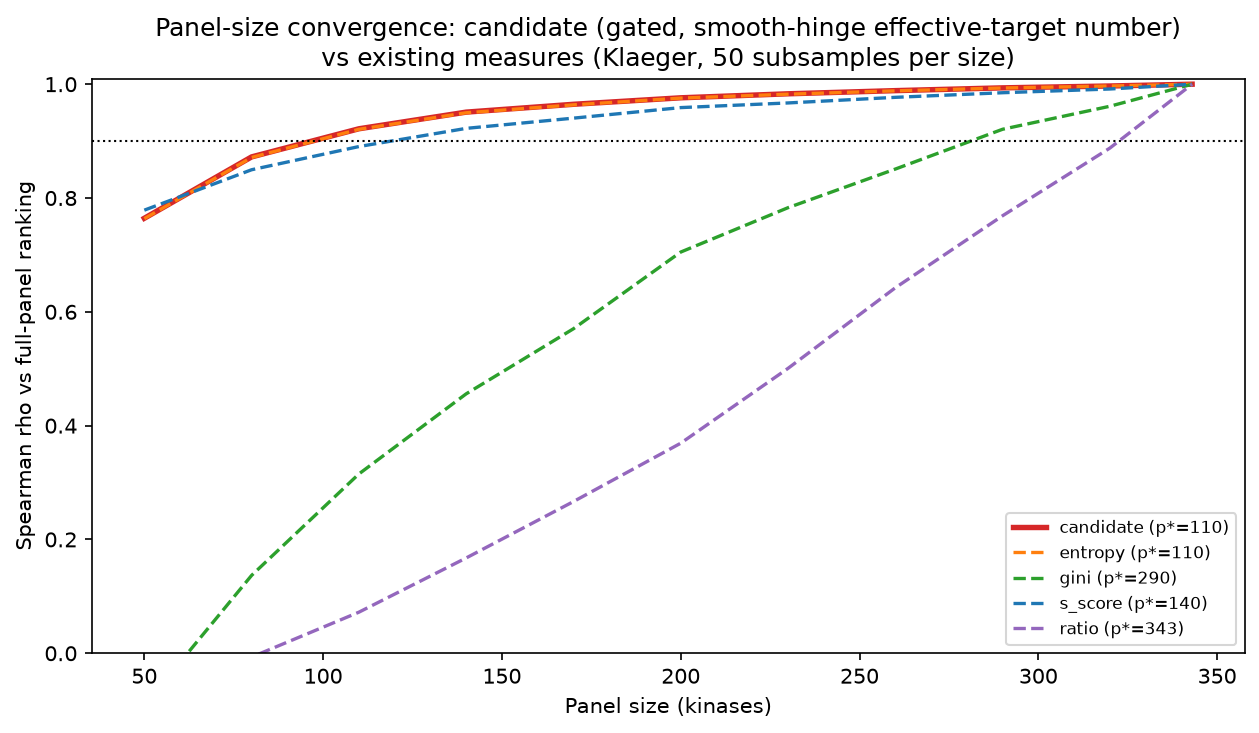
\includegraphics[width=\textwidth]{figures/candidate_panel_convergence}
  \caption{Panel-size convergence of the candidate measure compared with the four
           existing definitions, on the two sparse-coverage datasets (Klaeger,
           left; Metz, right; 50 random subpanels per size).
           Curves show the mean Spearman correlation between the ranking computed
           on a random subpanel and the full-panel ranking; $p^*$ (legend) is the
           smallest panel reaching mean $\rho > 0.90$.}
  \label{fig:candidate}
\end{figure}

\section{Discussion}
\label{sec:discussion}

The central finding of this work is that existing kinase inhibitor selectivity
definitions do not measure the same quantity.
The ratio definition and the distribution-based family (S-score, entropy, Gini)
produce substantially different compound rankings (cross-family
$r = 0.14$--$0.62$ across four datasets, versus within-family $r > 0.72$), and
the sources of disagreement are mechanistically interpretable rather than random.
This has practical consequences: a compound that ratio-based analysis designates
as selective may be designated as moderately promiscuous by entropy-based
analysis, and vice versa, depending on the shape of its binding profile.
Go/no-go decisions in early drug discovery are routinely made on the basis of
selectivity assessments without a principled choice of selectivity definition.

The clustering of definitions into two families
reflects a difference in what is being measured.
Distribution-based definitions ask: how concentrated is the compound's binding
activity across the full profiled kinome?
The ratio definition asks: how much more potently does the compound bind its
primary target than a specified off-target?
The selectivity measure discrepancy is most pronounced 
for compounds with one clearly dominant target that also
bind many kinases at moderate affinity (Type~3 profiles in our taxonomy).
For such compounds, ratio-based methods report high selectivity while
distribution-based methods report moderate promiscuity.
The required properties proposed in the Required Properties section are an
attempt to express what it means for a compound to be selective in a way that is
precise enough to assess candidate selectivity definitions formally.

This coexistence has a historical explanation.
In classical pharmacology and analytical chemistry, selectivity is inherently
pairwise. IUPAC formalizes it as a selectivity coefficient, the ratio of
binding constants for an analyte and an interferent\cite{IUPAC2001}, and
ratio measures entered kinase profiling on that basis.
Kinome-wide profiling, however, poses a distributional question: how
concentrated is a compound's binding across hundreds of kinases?
Entropy and Gini were introduced because ratio measures are ill-suited to it, since
they discard all but two points of a 300--500 kinase profile. 


\subsection{Practical Recommendations}

Pending a formal resolution, three practical recommendations follow from our
findings.
First, D1 (reliability threshold) should be adopted as a reporting
standard.
Compounds with no detected binding above the assay detection floor should not
receive selectivity scores, or should have their scores explicitly flagged as
unreliable.
Of the 222 Klaeger compounds, 16 (7.2\%) fall into this category and currently
receive scores that are indistinguishable from noise.

Second, selectivity assessments should report the sensitivity of rankings to
parameter choice rather than a single score at a single parameter value.
Our analysis shows that rank standard deviation across the parameter sweep is a
compound-specific, interpretable quantity that identifies which compounds have
robust selectivity assessments and which do not.
This is analogous to reporting confidence intervals in statistical estimation.

Third, when comparing selectivity across studies that use different definitions,
the comparison should be restricted to the subset of compounds and parameter
values for which the definitions agree.
The high within-family correlations ($r > 0.72$) suggest that S-score, entropy,
and Gini are interchangeable for most purposes when parameters are chosen
consistently. This is an empirical observation rather than a preset adequacy
bar: $r = 0.72$ is the lowest within-family correlation we observed (Klaeger
S-score vs.\ Gini, Table~\ref{tab:correlations}), and it measures a different
property than the $\rho > 0.90$ criterion used in the panel-size analysis
below. The former measures how similarly two distinct definitions rank compounds
on the full panel; the latter measures how similarly the same definition ranks
compounds on a subpanel versus the full panel. The
within-family agreement is measured on the complete kinome, and the panel-size
analysis shows that the Gini coefficient can diverge from the entropy and
S-score on the smaller panels used in practice (on Klaeger it requires roughly
290 of 343 kinases to recover its full-panel ranking, against 110 for
entropy and the S-score). The three measures should therefore be treated as
interchangeable only when compared on panels of similar, near-complete coverage.
Ratio-based measures, in turn, should not be compared directly with
distribution-based measures at any panel size without acknowledging the
conceptual distinction.

\subsection{Limitations}

The analysis covers four profiling datasets spanning three assay technologies
and two readout types, but these still represent a fraction of the chemical and
kinase space relevant to drug discovery.
The assay technologies are not directly comparable in absolute terms --- the
active-compound fractions differ across datasets. As a consequence,
our analysis
relies on within-dataset rank comparisons rather than cross-dataset absolute
scores.
The consistency of the two-family structure and the instability predictors
across all four datasets indicates that the findings are not artifacts of a
single assay platform. However, findings should still be interpreted in light of
these technological differences.
Our comparison is also restricted to four widely used, historically
established definitions. Bosc et al.'s window score and ranking
score\cite{Bosc2017} were not included, but a check on the same four datasets
confirms both correlate with the ratio family (Spearman $r = 0.80$--$0.96$)
rather than forming a distinct third cluster.
The CATDS score\cite{Klaeger2017}, historically classified alongside the
ratio-based measures, was also not implemented directly. Unlike $R(k)$, CATDS
normalizes each target's binding reduction by the sum of reductions across the
entire panel rather than comparing to a single off-target, a construction it
shares with the distribution-based family rather than with $R(k)$. A proxy
computed from our baseline-subtracted affinity profiles, in place of the raw
concentration-response data CATDS requires, correlates more strongly with Gini
and entropy than with $R(k)$ on Klaeger, consistent with this structural
reading. We did not add it as a fifth measure: the distribution family is
already represented by three members, and CATDS appears to be an additional
instance of the same underlying construct rather than an independent
perspective (see repository for results).

A further axis of platform dependence that this analysis does not examine is
cell-based versus cell-free profiling. Recent work shows that selectivity
classifications for the same compounds can differ substantially between
biochemical binding panels and cellular target-engagement assays. For example, several
type II (DFG-out-binding) inhibitors show cellular interactions that
cell-free assays miss\cite{Binder2026}. A plausible contributor, not established
by that work, is that cell-free panels often use truncated or constitutively
active kinase-domain constructs, which cannot adopt the DFG-out state.

We also examined whether in vitro selectivity predicts clinical toxicity,
correlating the selectivity rankings of the FDA-approved Klaeger compounds with
FAERS adverse-event rates ($n = 46$) and FDA-label discontinuation rates
($n = 33$).
None of the rate-based outcomes were significantly associated with selectivity
under any definition (all $|r| < 0.17$, all $p > 0.27$).
The only nominal signal is a weak correlation between raw FAERS report counts and
the ratio ranking ($r = 0.31$, $p = 0.035$), which most likely reflects
prescription volume rather than toxicity.
We do not read the absence of a rate-based association as evidence that
selectivity and toxicity are unrelated. FAERS report counts mostly track how
often a drug is prescribed, and label discontinuation depends on the patient
population treated for each indication, so neither can isolate the effect of
selectivity.
A proper test would require indication-stratified, treatment-related
adverse-event rates from controlled trials with matched comparators, which are
not available in standardized form across these drugs.

The four properties proposed above are necessary
conditions motivated by empirical failure modes.
The candidate measure shows that they are jointly satisfiable, but they are not
proven to be sufficient to uniquely characterize a selectivity measure, and we do
not show that they single out a measure of the candidate's form.
The satisfaction assessments in Table~\ref{tab:desiderata} are based on
analysis of the functional forms of each definition together with the empirical
checks of this study. A formal proof of satisfaction or violation for each
property--definition pair is left for future work.

\section{Conclusion}
\label{sec:conclusion}

We have shown that commonly used kinase inhibitor selectivity definitions
cluster into two families that measure fundamentally different properties of
binding profiles. We also showed that rank instability within and between families is
mechanistically predictable from binding profile shape, and that three
structurally distinct sources of instability can be identified and
characterized.
These findings motivate four required properties that any well-formed selectivity measure
should satisfy: a reliability threshold
condition, bounded gap sensitivity, distributional consistency, and monotonicity
under weak off-target addition.

No existing definition satisfies all four simultaneously, but we show that a
gated, smooth-hinge effective-target number does. We demonstrate that it recovers its
full-panel ranking from roughly a third of a typical panel, and that it is
part of a whole family of candidate definitions satisfying the four properties.
However, our featured candidate measure is close to identical to the
entropy measure in terms of performance on the given datasets, and
looking for a significantly better measure within the candidate family is future work,
likely requiring additional datasets.
Establishing additional properties that characterize a selectivity measure
uniquely, as Shannon's axioms do for entropy, is a natural next step.

The immediate practical implication is that selectivity assessments should
report the sensitivity of rankings to parameter choice, and should explicitly
flag compounds with no binding above the detection threshold as unreliable.
The longer-term implication is that the field needs a principled basis for
choosing among selectivity definitions.
The need for a principled measure is not specific to selectivity. 
As future and ongoing work, we are developing a general
measurement-theoretic framework for defining and comparing the competing
measures of one concept, reporting where they agree and which pairs they
leave undecided, with kinase selectivity as one instance alongside cases
as varied as biological age and variant effect prediction.



\begin{acknowledgement}
The author thanks the developers of the Davis, Klaeger, Anastassiadis, and Metz
datasets for making their data publicly available.
The author used Claude (Anthropic, claude.ai), a large language model assistant,
during the preparation of this manuscript.
Specifically, Claude was used to assist with: data analysis code development and
debugging in Python; literature search and identification of related work;
drafting and editing of manuscript text; and research planning and
interpretation of results.
All scientific conclusions, the conceptual framework, the required properties proposed in the
Required Properties section, and the final manuscript content were developed, verified, and
approved by the author.
The author takes full responsibility for the accuracy and integrity of all
content in this work.
The use of Claude does not transfer any rights over the content of this manuscript
to Anthropic or any third party.
\end{acknowledgement}

\section*{Data and Software Availability}
All data and software used in this study are publicly available.
The Davis kinase inhibitor profiling dataset is available at
\url{https://github.com/dingyan20/Davis-Dataset-for-DTA-Prediction}.
The Klaeger et al.\ dataset is available as supplementary data to the
original publication (Science, 2017, \url{https://doi.org/10.1126/science.aan4368}).
The Anastassiadis et al.\ (\emph{Nat. Biotechnol.} 2011) and Metz et al.\
(\emph{Nat. Chem. Biol.} 2011) datasets are available as supplementary data to
their original publications
(\url{https://doi.org/10.1038/nbt.2017}; \url{https://doi.org/10.1038/nchembio.530}).
All analysis scripts, processed data files, and the \LaTeX\ source for
this manuscript are available at
\url{https://github.com/polinavino/kinase-selectivity-definitions};
this repository includes the code and full per-definition results for the
secondary clinical-outcome analysis (FAERS adverse-event report rates and
FDA-label discontinuation rates for the FDA-approved Klaeger compounds,
with the openFDA queries used).
No confidential data were used in this study.
All results reported in this manuscript are fully reproducible from the
publicly available data and code.
A preprint of this manuscript is available on ChemRxiv at
\url{https://doi.org/10.26434/chemrxiv.15001618/v1}.

\section*{Funding}
This research received no specific grant from any funding agency in the public,
commercial, or not-for-profit sectors.

\section*{Conflict of Interest}
The author declares no conflict of interest.

\bibliography{references}

\end{document}
